Now, we measure bandwidth and latency overhead of {\sys} for two different applications using our traffic shaping simulator (see \Cref{sec:eval-simulator}).
Similar to previous section, we use two case studies: a video streaming application and a web service application. 
In both applications, a client initiates a bidirectional communication with the server to retrieve content.
We apply traffic shaping in both directions, customizing the parameters to match the traffic characteristics specific to each direction of communication.


\subsection{Case Study: Video Streaming}\label{subsec:eval-bw-video}
\begin{figure}[t]
  \centering
  \begin{subfigure}{0.49\columnwidth}
      \centering
      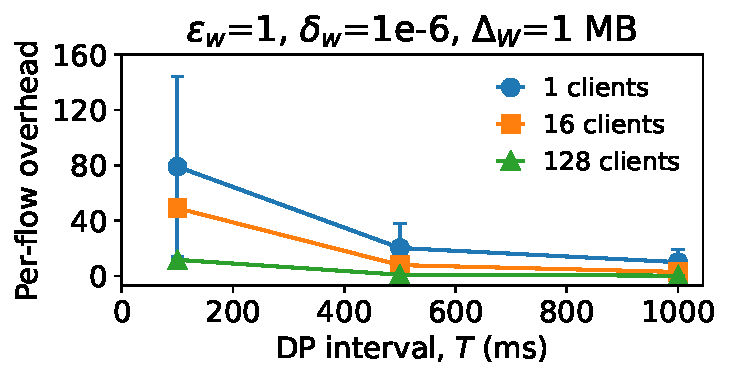
\includegraphics[width=\textwidth]{plots/overhead_vs_dp_interval_video.pdf}
      \caption{BW overhead vs DP interval}
      \label{fig:video-overhead-vs-dpInt}
  \end{subfigure}
  \hfill
  \begin{subfigure}{0.49\columnwidth}
      \centering
      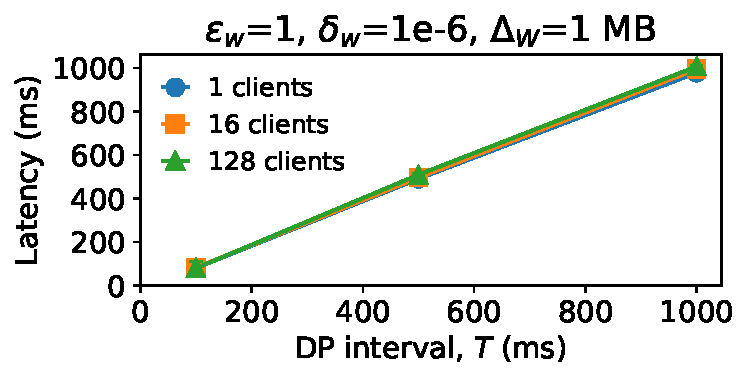
\includegraphics[width=\textwidth]{plots/latency_vs_dp_interval_video.pdf}
      \caption{Latency vs DP interval}
      \label{fig:video-latency-vs-dpInt}
  \end{subfigure}
  \caption{Video Streaming; Bandwidth and latency overhead for different values of DP interval.
  }
\end{figure}

We examine the effect of different privacy settings on bandwidth overhead for video streaming clients.
We run experiments with three values of the DP measurement interval $\dpintvl$ for the server:
100ms, 500ms, and 1s, and we use $\ssens = 1 MB$ and $\varepsilon_{\winlen} = 1$.
For all experiments, we set the DP parameters for client request traffic as follows: $\ssens = 200$~bytes, $\winlen = 1s$, $\dpintvl = 100ms$, and $\varepsilon_{\winlen} = 1$.
For the server responses, we configure DP parameters as follows: $\ssens = 1 MB$~bytes, $\winlen = 5s$, $\dpintvl = 1 s$, and $\varepsilon_{\winlen} = 1$.
We use different set of parameters for communication from server to client and vice versa due to the different characteristics of traffic in each direction.
Periodically, at intervals of 5 seconds, the client sends a small web request  to the server to download the next video segment. 
In the reverse direction, the server transmits segments to the client one by one.
Compared to the small client requests, segments are larger and have a bursty traffic pattern.
As the client requests each segment preemptively, as long as the server delivers the next segment within 5 seconds, the client can play video seamlessly. 
We run experiments with 1, 16, and 128 video clients; each client requests one video randomly selected from the dataset.
For each set of configurations, we measure the per-flow relative bandwidth overhead for the video streams in the simulator.
We use {\sys}'s artifact to measure the latency of each segment.
Finally, we measure the average response latency for individual video segments with {\sys}'s artifact~\cite{netshaper_repo}.





\paragraph{Bandwidth overhead.}
\Cref{fig:video-overhead-vs-dpInt} shows the average per-flow relative bandwidth overhead as a function of DP interval and for varying number of clients.
The relative bandwidth overhead of a video is the number of dummy bytes transmitted normalized to the size of the unshaped video stream.
The error bars show the standard deviation in latency and bandwidth overhead.
The relative overhead decreases as the DP interval increases, as the DP shaping mechanism introduces noise to the queue size with each DP measurement.
A larger DP interval means that the DP shaping mechanism introduces noise less frequently, leading to a smaller overhead. 
Besides that, \Cref{fig:video-overhead-vs-dpInt} represents that the bandwidth overhead is amortized when there are multiple concurrent streaming clients.
Overall, {\sys}'s shaping can secure video streams with low bandwidth overheads.

\paragraph{Latency Overhead}
We measure the latency for different values of $\dpintvl$.
\Cref{fig:video-latency-vs-dpInt} shows that, for all values of $\dpintvl$, the video segments can be downloaded well within 5s. 
Besides that, the results show the trade-off between latency and bandwidth.
A larger DP measurement interval implies increased download latency but fewer DP measurements and less noise added to the queue size, resulting in reduced bandwidth overhead.







\subsection{Case Study: Web Service}\label{subsec:eval-bw-web}
\begin{figure}[t]
  \centering
  \begin{subfigure}{0.49\columnwidth}
      \centering
      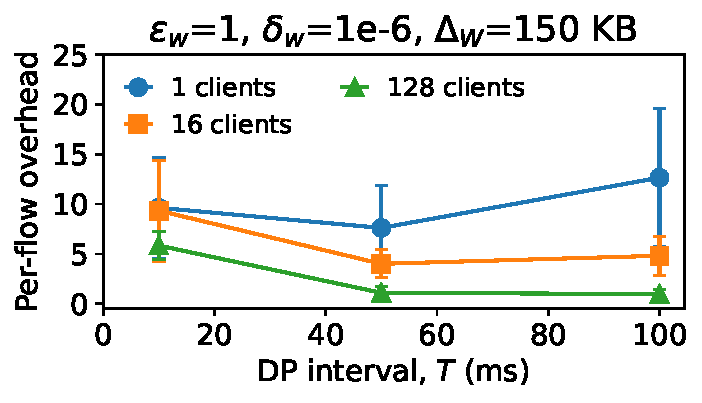
\includegraphics[width=\textwidth]{plots/overhead_vs_dp_interval_web.pdf}
      \caption{BW overhead vs DP interval}
      \label{fig:web-overhead-vs-dpInt}
  \end{subfigure}
  \hfill
  \begin{subfigure}{0.49\columnwidth}
      \centering
      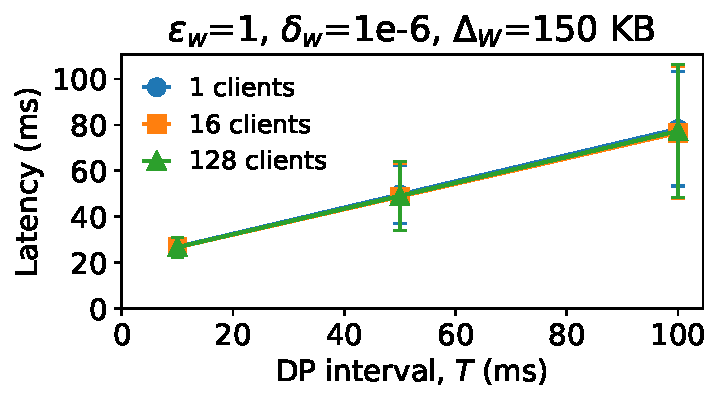
\includegraphics[width=\textwidth]{plots/latency_vs_dp_interval_web.pdf}
      \caption{Latency vs DP interval}
      \label{fig:web-latency-vs-dpInt}
  \end{subfigure}
  \caption{Web Service; Bandwidth and latency overhead for different values of DP interval.
  }
\end{figure}
Now, we examine the effect of different privacy settings on bandwidth overhead for a web service.
As we mentioned in previous section, we expect the length of DP interval ($T$) affects end-to-end latency.
We choose smaller values for $\dpintvl$ for web service compared to video streaming applications as web applications are delay-sensitive.
We assess latency by measuring the time it takes to receive each webpage.
For the server responses, we use three DP measurement intervals, $\dpintvl$: 10 ms, 50 ms, 100 ms, and the other parameters are: $\ssens = 150 KB$, $\winlen = 1s$, and
$\varepsilon_{\winlen} = 1$.
For the client requests, we use $\ssens = 200 B$, $winlen = 1s$, and $\varepsilon_{\winlen} = 1$.
We run experiments with 1, 16, and 128 video clients; each client requests a random webpage from the dataset.



\paragraph{Bandwidth overhead.}
\Cref{fig:web-overhead-vs-dpInt} shows the average per-web page relative bandwidth overhead, across all web page requests.
The bandwidth overhead for web traffic first reduces with increasing DP measurement interval from 10ms to 50ms, but interestingly, it increases again
with an interval of 100ms.
The reason behind this is that for small web pages, a 100ms DP interval exceeds the entire time needed to download them.
As a result, additional overhead is incurred due to the padding of traffic in the 100ms intervals.
Similar to video streaming applications, when there are multiple concurrent requests from clients, the relative bandwidth overhead tends to decrease.

\paragraph{Latency Overhead}
\Cref{fig:web-latency-vs-dpInt} shows the latency for different values of $\dpintvl$.
Similar to video streaming, the latency increases with larger values of DP interval.
As web services are latency-sensitive, we use smaller values of DP interval in this experiment. 
Based on this figure, the optimal value of DP interval for our web service is $\dpintvl = 50 ms$. 
With this value, the overhead is minimized, and a latency of 50 ms remains acceptable for web applications. 


\section{Comparison with Prior Techniques}\label{sec:eval-comparison-others}


\begin{figure}[t]
  \centering
  \begin{subfigure}{0.49\columnwidth}
      \centering
      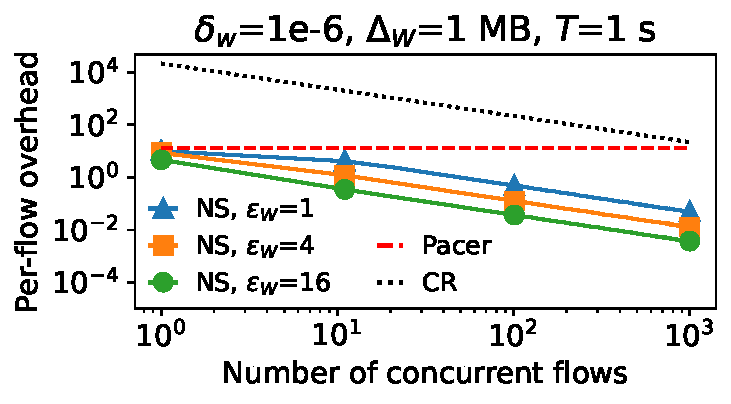
\includegraphics[width=\textwidth]{plots/overhead_vs_number_of_traces_video_loglog.pdf}
      \caption{Video streaming.}
      \label{fig:video-overheads-compare}
  \end{subfigure}
  \hfill
  \begin{subfigure}{0.49\columnwidth}
      \centering
      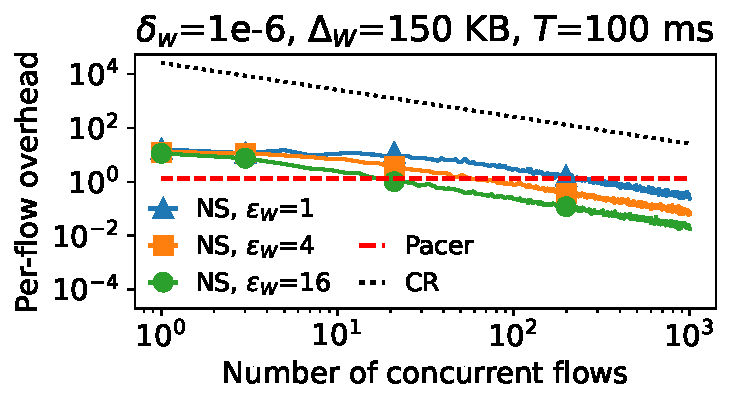
\includegraphics[width=\textwidth]{plots/overhead_vs_number_of_traces_web_loglog.pdf}
      \caption{Web service.}
      \label{fig:web-overheads-compare}
  \end{subfigure}
  \caption{Relative bandwidth overheads of {\sys} ({\ns}), constant
      shaping ({\constshape}), and Pacer.
  }
\end{figure}

\paragraph{Video Streaming.}
\Cref{fig:video-overheads-compare} shows the per-flow relative bandwidth overhead of {\sys} ({\ns}) for the video streaming application as a function of the number of concurrent flows and for different values of $\varepsilon_{\winlen}$.
Except $\varepsilon_{\winlen}$, we use the same of parameters that we proposed in \Cref{sec:eval-bw}.
We also compare with the overheads~that would be incurred due to constant rate
shaping ({\constshape}) and~Pacer \cite{mehta2022pacer} (see \Cref{subsubsec:background-defenses-pacer}), a state-of-the-art traffic shaping system.

For {\constshape}, we configure the peak load for the video service corresponding to
transmitting 1.7MB in 5s intervals, which is corresponding to transmitting the largest segment size in our video dataset. In other words, the {\constshape} mechanism always sends data at the maximum rate required to send a segment in our dataset.
In Pacer, for video service, we pad a segment at the $i$\textsuperscript{th} index
in a video stream to the largest segment size at that index across all videos in the dataset. 
Even with the lowest privacy loss, $\varepsilon_{winlen}=1$, {\ns} adds the same level of overhead as Pacer and 3 orders of magnitude less overhead than {\constshape}.  
Besides that, {\ns} can amortize the overhead
among multiple concurrent streams within the tunnel without compromising privacy.

\paragraph{Web Service.}
\Cref{fig:web-overheads-compare} shows the per-flow relative bandwidth overhead of {\sys} ({\ns}) for a web service as a function of the number of concurrent flows for different values of $\varepsilon_{\winlen}$.
We configure the remaining parameters at the same values as previously mentioned in \Cref{sec:eval-bw}.
Similar to the video streaming, for the web service, we compare {\sys} ({\ns}) Pacer and constant rate shaping ({\constshape}).
For {\constshape}, we configure the peak load for web service corresponding to
transmitting 57KB in every 50ms, which is corresponding to transmitting the largest web page in our dataset.
For web services, Pacer pads all web pages to the largest page size, which is 147KB in our dataset.
Similar to the video streaming case study, {\ns} introduces overheads that are several orders of magnitude smaller compared to {\constshape}.
However, {\ns} requires more than 20 flows to achieve lower overhead than Pacer.
Pacer shapes server traffic only upon receiving a client request and does not
shape client traffic. 
Thus, it leaks the timing and shape of client requests, which could potentially reveal information about the server responses \cite{chen2010reality}.
{\sys} shapes traffic in both directions, which incurs higher overhead at the cost of stronger privacy than Pacer. 